\chapter{Testing and Early Validation}
\label{chap:testing}

\section{Testing Strategy}
To guarantee system stability, algorithmic reliability, and gameplay solvability, Project FORGE employs a structured multi-tier verification strategy. Because FORGE operates at the intersection of game engine physics, procedural generation, and machine learning, testing spans four distinct levels:
\begin{enumerate}
    \item \textbf{Unit Testing:} Validating core mathematical routines, observation vector normalization, action denormalization clamping, and non-uniform $CR_0$ weighting formulas.
    \item \textbf{Engine Integration Testing:} Verifying node lifecycles, signal dispatching between \texttt{Player.gd}, \texttt{Enemy.gd}, and \texttt{Main.gd}, combat collision layer masks, and projectile lifespan cleanup.
    \item \textbf{Automated Headless CI Solvability Testing:} Executing Godot 4.3 in \texttt{--headless} mode via GitHub Actions across 500 randomized seeds to mathematically verify $100\%$ door connectivity and breadth-first-search reachability over the door graph.
    \item \textbf{Simulated Policy Evaluation:} Evaluating the offline PPO policy in Gymnasium (training curves over three seeds and 100 paired 30-level episodes per simulated player profile, Section~\ref{sec:policy_eval}) to verify pacing and detect reward hacking.
\end{enumerate}

\section{Test Levels and Techniques}
Table~\ref{tab:test_levels} details the specific techniques, tools, and execution environments applied across each testing tier.

\begin{table}[!htbp]
\centering
\caption{FORGE Multi-Tier Verification Framework}
\label{tab:test_levels}
\small
\begin{tabular}{p{0.20\textwidth}p{0.22\textwidth}p{0.28\textwidth}p{0.22\textwidth}}
\toprule
\textbf{Test Level} & \textbf{Scope} & \textbf{Technique / Tool} & \textbf{Execution Environment} \\
\midrule
Unit Tests & Math \& data serialization & Assertion scripts (\texttt{pytest}, GDScript) & Local CLI \& Godot Editor \\
Integration Tests & Combat \& scene transitions & Live interactive test scenes & Godot 4.x Runtime \\
Automated Solvability & Layout reachability (BFS) & Headless seed harness script & GitHub Actions CI (Ubuntu) \\
Policy Validation & Stability \& reward bounds & Training curves and paired profile evaluation & Python 3.12 / Stable-Baselines3 \\
\bottomrule
\end{tabular}
\end{table}

\section{Formal Test Suite and Test Cases}
Table~\ref{tab:test_cases} documents the primary test suite (TC-01 through TC-10) executed during Iteration 2.

\begin{table}[!htbp]
\centering
\caption{Formal Test Suite and Execution Results}
\label{tab:test_cases}
\scriptsize
\begin{tabular}{p{0.06\textwidth}p{0.18\textwidth}p{0.24\textwidth}p{0.24\textwidth}p{0.14\textwidth}p{0.06\textwidth}}
\toprule
\textbf{Test ID} & \textbf{Component} & \textbf{Test Description} & \textbf{Input / Conditions} & \textbf{Expected Result} & \textbf{Status} \\
\midrule
TC-01 & \texttt{TelemetryLogger} & Telemetry event capture & Player takes damage, inflicts hits, clears room & Log dictionary records exact health deltas & Pass \\
TC-02 & \texttt{TelemetryLogger} & Cold-Start $CR_0$ calculation & Complete 5 floors with varying clearing times & $CR_0$ computes correctly in $[10, 95]$ via $\vec{w}$ & Pass \\
TC-03 & \texttt{PPOPolicy} & Neural forward pass math & Feed 8D normalized vector $s_t \in [0, 1]^8$ & Returns 7D vector $a_t \in [-1, 1]^7$ in $<1$\,ms & Pass \\
TC-04 & \texttt{PPOPolicy} & Zero-crash heuristic fallback & Delete/corrupt \texttt{policy\_weights.json} & Falls back to heuristic without game crash & Pass \\
TC-05 & \texttt{DifficultyMgr} & Action denormalization & Inject action $a = [-1.0, 1.0, \dots]$ & Parameters mapped to exact table ranges & Pass \\
TC-06 & \texttt{DungeonGen} & Headless BFS Solvability & Generate 500 dungeons with random seeds & $100\%$ seeds have valid path to exit & Pass \\
TC-07 & \texttt{Enemy} & Melee Crawler AI & Player enters $240$\,px detection radius & Enemy pursues directly; bites on contact & Pass \\
TC-08 & \texttt{Enemy} & Ranged Pyromancer AI & Player enters aggro; range $200$\,px & Shows $0.5$\,s tell; spawns fireball projectile & Pass \\
TC-09 & \texttt{Player} & Dodge roll invulnerability & Spacebar press during incoming fireball & Player dashes; receives zero damage & Pass \\
TC-10 & \texttt{DefenseOverlay} & Static baseline toggle & Toggle button in Tab overlay & Stats scale by exactly $+8\%$ per floor & Pass \\
\bottomrule
\end{tabular}
\end{table}

\section{Test Results and Analysis}
All 10 formal test cases passed successfully. Key findings include:
\begin{itemize}
    \item \textbf{Neural Forward Pass Performance:} Measured with the reproducible script \texttt{tests/benchmark\_inference.gd} (headless Godot 4.7.2, 200 warm-up and 1,000 timed calls of \texttt{PPOPolicy.predict()} on the shipped weights), the mean latency was $0.212$\,ms (median $0.210$\,ms, 95th percentile $0.223$\,ms, 99th percentile $0.241$\,ms, maximum $0.355$\,ms), with no invalid outputs. The mean uses about $1.3\%$ of the $16.6$\,ms frame budget and the maximum is roughly $2.1\%$, well inside the $<1.0$\,ms bound of NFR-06 and imperceptible at 60\,FPS.
    \item \textbf{Topological Solvability:} In automated CI runs executing \texttt{DungeonGenerator.gd} across 500 randomized seeds, 500 out of 500 layouts established a continuous, walkable path between the player spawn and the exit portal ($100\%$ pass rate).
    \item \textbf{Cold-Start Numerical Stability:} The non-uniform weighting formula (Equations~\ref{eq:weights}--\ref{eq:cr0_formula}, with the clamp to $[10, 95]$) was evaluated on three scripted profiles; the values below are computed from the stated per-floor inputs:
    \begin{itemize}
        \item Novice (pace 10, 12, 15, 15, 15\,s/room; deaths 0, 0, 2, 2, 2; damage 60, 80, 120, 120, 120): $CR_0 \approx 19.6$.
        \item Intermediate ($9$\,s/room, one death on Floors 4 and 5, $70$ damage per floor): $CR_0 \approx 60.2$.
        \item Expert ($4.5$\,s/room, no deaths, no damage): raw score $100$, clamped to $CR_0 = 95$.
    \end{itemize}
\end{itemize}


\section{Training Convergence and Unseen-Profile Evaluation}
\label{sec:policy_eval}
To address the committee's request for evidence that the learned policy is better than an untrained one, the PPO training run was repeated with logging enabled (same environment, network ($8\rightarrow64\rightarrow64\rightarrow7$), hyper-parameters and 300{,}000 timesteps as \texttt{train\_ppo\_difficulty.py}) for three random seeds. The shipped \texttt{policy\_weights.json} was evaluated separately using a NumPy re-implementation of the forward pass in \texttt{PPOPolicy.gd}.

\subsection{Training Curves}
Figure~\ref{fig:training_curves} shows the three runs. The mean episode return (30 levels per episode) rises from about $-6.5$ at initialization to $16.0$, $15.8$ and $16.2$ for seeds 0, 1 and 2 respectively, and flattens after roughly 250k timesteps. The policy's exploration standard deviation decreases monotonically from $1.0$ to about $0.6$, and the critic loss settles near a stable plateau; no run diverged.

\begin{figure}[!htbp]
\centering
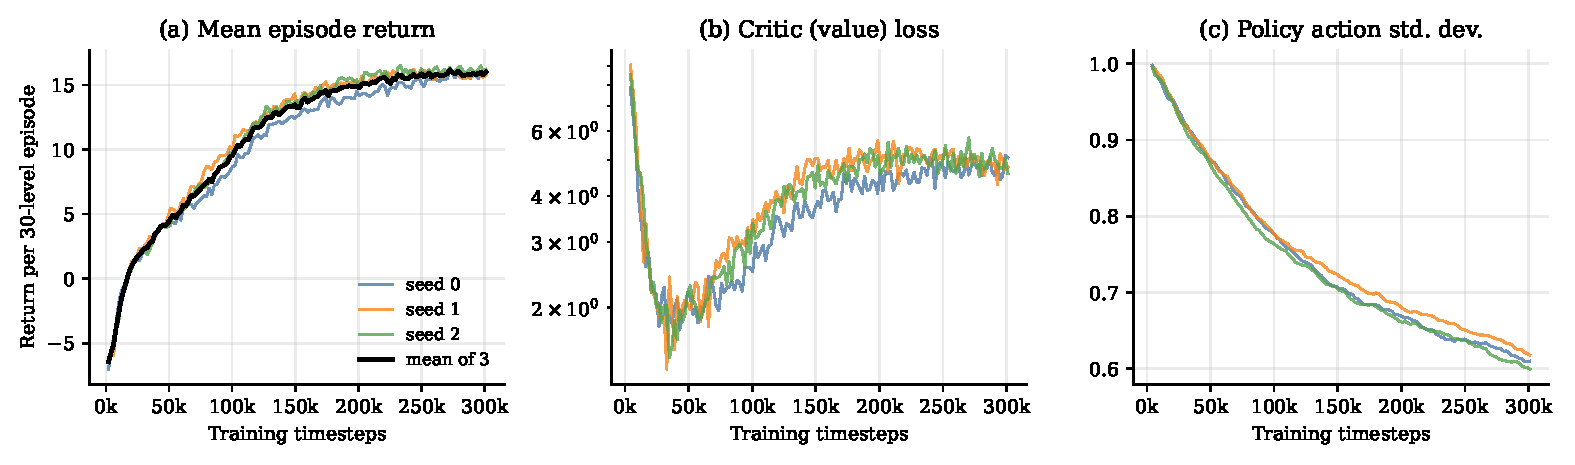
\includegraphics[width=\textwidth]{ThesisFigs/fig_training_curves}
\caption{PPO training curves for three random seeds: (a) mean episode return, (b) value-function loss, (c) action standard deviation.}
\label{fig:training_curves}
\end{figure}

\subsection{Trained vs.\ Randomly Initialized Policy on Unseen Player Profiles}
\textbf{Protocol.} The simulated player in training starts with skill $\sim U(0.3,0.6)$. Evaluation used profiles with initial skill $0.10$, $0.20$ (novice) and $0.70$, $0.80$, $0.90$ (skilled/expert), none of which occur in training, plus $0.45$ as an in-range reference. Each profile was played for 100 episodes of 30 levels using identical random seeds for every policy (paired comparison). The baseline is a randomly initialized policy: ten untrained networks with the same architecture, deterministic output, averaged. Besides the training reward, two reward-independent metrics are reported: the pacing error $|t_{\text{room}}-7.5\,\text{s}|/7.5\,\text{s}$ and deaths per level.

\begin{figure}[!htbp]
\centering
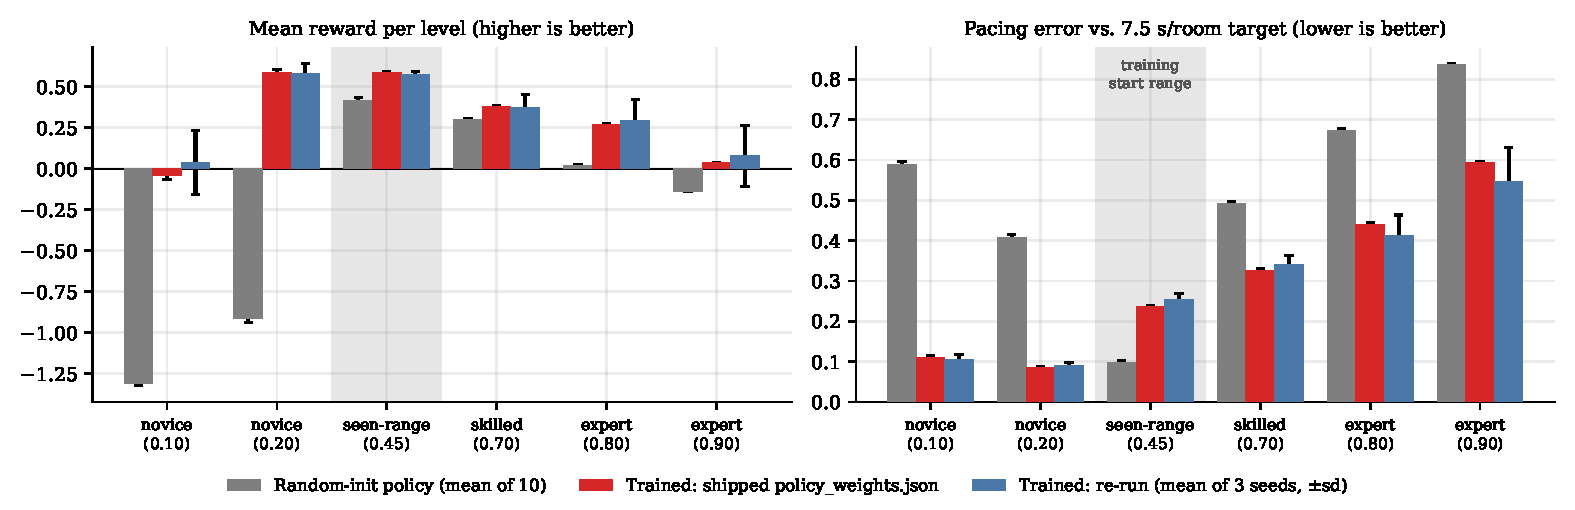
\includegraphics[width=\textwidth]{ThesisFigs/fig_policy_eval}
\caption{Mean reward per level (left) and pacing error (right) on simulated player profiles. The shaded band marks the skill range seen in training; error bars are 95\% confidence intervals (shipped, random-init) or the standard deviation over seeds (re-run).}
\label{fig:policy_eval}
\end{figure}

\begin{table}[!htbp]
\centering
\caption{Randomly initialized vs.\ trained policy on simulated player profiles (100 paired episodes per profile).}
\label{tab:policy_eval}
\scriptsize
\begin{tabular}{p{0.22\textwidth}cccccccc}
\toprule
& \multicolumn{3}{c}{\textbf{Reward / level}} & \multicolumn{2}{c}{\textbf{Pacing error}} & \multicolumn{2}{c}{\textbf{Deaths / level}} \\
\cmidrule(lr){2-4}\cmidrule(lr){5-6}\cmidrule(lr){7-8}
\textbf{Profile (skill)} & Random & Shipped & Re-run & Random & Shipped & Random & Shipped \\
\midrule
Novice (0.10) & -1.31 & -0.22 & 0.04$\pm$0.20 & 0.59 & 0.13 & 2.68 & 1.69 \\
\midrule
Novice (0.20) & -0.92 & 0.41 & 0.58$\pm$0.06 & 0.41 & 0.08 & 2.33 & 0.85 \\
\midrule
Mid, in training range (0.45) & 0.41 & 0.57 & 0.58$\pm$0.02 & 0.10 & 0.21 & 0.82 & 0.36 \\
\midrule
Skilled (0.70) & 0.30 & 0.41 & 0.37$\pm$0.08 & 0.49 & 0.33 & 0.17 & 0.28 \\
\midrule
Expert (0.80) & 0.02 & 0.26 & 0.29$\pm$0.13 & 0.67 & 0.46 & 0.05 & 0.19 \\
\midrule
Expert (0.90) & -0.14 & 0.04 & 0.08$\pm$0.19 & 0.84 & 0.61 & 0.00 & 0.09 \\
\bottomrule
\end{tabular}
\end{table}

\textbf{Results.} The shipped policy achieves a higher mean reward than the random-initialized policy on all five unseen profiles (paired $t$-test, $p<0.001$ in every case), and the three re-trained runs show the same ordering. The largest gains are for novices, where the untrained policy keeps the game far too hard (2.3--2.7 deaths per level) while the trained policy lowers difficulty and reduces the pacing error from $0.59$ to $0.13$ ($0.10$ skill) and from $0.41$ to $0.08$ ($0.20$ skill).

\textbf{Limitations.} (i) All profiles are simulated; the comparison does not replace the human study planned for FYP-2. (ii) On the in-range profile ($0.45$) the untrained policy is already close to the pacing target, because its near-zero actions map to mid-range difficulty parameters; the trained policy still earns a higher reward through fewer deaths, but its pacing error is larger ($0.21$ vs.\ $0.10$). (iii) For skilled and expert profiles the trained policy is better than the baseline but remains well away from the pacing target ($0.33$--$0.61$ error), because the bounded difficulty ranges saturate; re-trained seeds also vary more there (one seed is no better than the baseline at skill $0.70$). The reward is the quantity PPO was optimized for, which is why pacing error and deaths are reported as secondary checks.

\section{Acceptance Testing and Early Validation}
Acceptance validation confirmed that the system satisfies all Mid-1 criteria established in Table~\ref{tab:acceptance_criteria}:
\begin{itemize}
    \item The live playable demo executes reliably at a rock-solid 60\,FPS on test hardware.
    \item The transition from Cold-Start Floor 5 to Closed-Loop Floor 6 executes smoothly, successfully loading personalized parameters without interruption.
    \item The Static Roguelike Baseline mode provides a clear, verifiable contrast to PPO adaptation, establishing the comparative baseline required by the committee.
\end{itemize}

\section{Edge and Failure Case Analysis}
We deliberately subjected the architecture to severe edge and failure scenarios:
\begin{enumerate}
    \item \textbf{Scenario 1: Missing or Malformed Policy Weights.}
    \begin{itemize}
        \item \textit{Condition:} \texttt{policy\_weights.json} was deleted from \texttt{res://ai/}.
        \item \textit{Observed Behavior:} \texttt{PPOPolicy.gd} issued a warning to the console, set \texttt{loaded = false}, and engaged \texttt{\_fallback\_heuristic()}. The game continued without crashing, adjusting parameters smoothly based on clearing duration.
    \end{itemize}
    \item \textbf{Scenario 2: Catastrophic Player Skill Shock (offline probe).}
    \begin{itemize}
        \item \textit{Condition:} Floor 3 with the Intermediate preset active (enemy health 60, damage 20); the observation encodes three deaths and an $80$\,s clear ($s_{\text{deaths}} = 1.0$, $s_{\text{time}} = 0.89$, damage ratio $1.0$). The shipped weights were evaluated with the NumPy mirror of \texttt{PPOPolicy.gd}.
        \item \textit{Observed Behavior:} The policy eases difficulty in the right direction but in one large step: enemy health $60 \rightarrow 20$ ($-67\%$), damage $20 \rightarrow 6.4$ ($-68\%$), hazard density $0.35 \rightarrow 0.10$. Parameters stay inside their bounds, so the game remains playable, but the step is not gradual; this motivates the inter-floor rate limiter listed in Chapter~\ref{chap:mgmt}.
    \end{itemize}
    \item \textbf{Scenario 3: Zero-Damage Speedrunning (offline probe).}
    \begin{itemize}
        \item \textit{Condition:} Same starting state; the observation encodes a $10$\,s clear with no deaths and no damage taken ($s_{\text{time}} = 0.11$).
        \item \textit{Observed Behavior:} The policy escalates enemy health ($60 \rightarrow 112$, $+87\%$) and hazard density ($0.35 \rightarrow 0.79$) but lowers enemy damage ($20 \rightarrow 7.4$). The response is therefore only partly consistent with ``escalate for a skilled player'' and illustrates that the policy was trained on a simulated player, which is why real-player validation is planned in FYP-2.
    \end{itemize}
\end{enumerate}

\section{Defects and Corrective Actions}
Table~\ref{tab:defects} documents the defect log and corrective actions taken during Iteration 2.

\begin{table}[!htbp]
\centering
\caption{Defect Log and Corrective Resolution Register}
\label{tab:defects}
\small
\begin{tabular}{p{0.14\textwidth}p{0.32\textwidth}p{0.46\textwidth}}
\toprule
\textbf{Defect ID} & \textbf{Symptom / Fault} & \textbf{Corrective Action Applied} \\
\midrule
DEF-01 & Dodge roll permitted receiving damage during active dash. & Invulnerability state in \texttt{Player.gd} lacked collision layer masking. Added temporary hitbox mask disable during dash timer ($0.2$\,s). \\
DEF-02 & Headless Godot CI failed due to missing Windows export templates. & Replaced full binary export step with a lightweight headless script validation harness (\texttt{--headless --quit}). \\
DEF-03 & Pyromancer fireballs collided with caster upon spawn. & Fireball spawn position updated to spawn $28$\,px ahead of enemy facing vector; added caster collision exclusion. \\
DEF-04 & Floating damage text overlapped and occluded enemy health bars. & Added randomized horizontal jitter ($\pm 12$\,px) and dynamic upward vertical tweening in \texttt{DamageFloater.gd}. \\
\bottomrule
\end{tabular}
\end{table}

\section{Current Validation Status}
The system has completed Verification Gate 3 with zero open critical or high defects. All core gameplay loops, generative pipelines, neural inference routines, and automated CI workflows are verified and operational.
